\documentclass[dvipsnames]{beamer}\usepackage[]{graphicx}\usepackage[]{color}
%% maxwidth is the original width if it is less than linewidth
%% otherwise use linewidth (to make sure the graphics do not exceed the margin)
\makeatletter
\def\maxwidth{ %
  \ifdim\Gin@nat@width>\linewidth
    \linewidth
  \else
    \Gin@nat@width
  \fi
}
\makeatother

\definecolor{fgcolor}{rgb}{0.345, 0.345, 0.345}
\newcommand{\hlnum}[1]{\textcolor[rgb]{0.686,0.059,0.569}{#1}}%
\newcommand{\hlstr}[1]{\textcolor[rgb]{0.192,0.494,0.8}{#1}}%
\newcommand{\hlcom}[1]{\textcolor[rgb]{0.678,0.584,0.686}{\textit{#1}}}%
\newcommand{\hlopt}[1]{\textcolor[rgb]{0,0,0}{#1}}%
\newcommand{\hlstd}[1]{\textcolor[rgb]{0.345,0.345,0.345}{#1}}%
\newcommand{\hlkwa}[1]{\textcolor[rgb]{0.161,0.373,0.58}{\textbf{#1}}}%
\newcommand{\hlkwb}[1]{\textcolor[rgb]{0.69,0.353,0.396}{#1}}%
\newcommand{\hlkwc}[1]{\textcolor[rgb]{0.333,0.667,0.333}{#1}}%
\newcommand{\hlkwd}[1]{\textcolor[rgb]{0.737,0.353,0.396}{\textbf{#1}}}%

\usepackage{framed}
\makeatletter
\newenvironment{kframe}{%
 \def\at@end@of@kframe{}%
 \ifinner\ifhmode%
  \def\at@end@of@kframe{\end{minipage}}%
  \begin{minipage}{\columnwidth}%
 \fi\fi%
 \def\FrameCommand##1{\hskip\@totalleftmargin \hskip-\fboxsep
 \colorbox{shadecolor}{##1}\hskip-\fboxsep
     % There is no \\@totalrightmargin, so:
     \hskip-\linewidth \hskip-\@totalleftmargin \hskip\columnwidth}%
 \MakeFramed {\advance\hsize-\width
   \@totalleftmargin\z@ \linewidth\hsize
   \@setminipage}}%
 {\par\unskip\endMakeFramed%
 \at@end@of@kframe}
\makeatother

\definecolor{shadecolor}{rgb}{.97, .97, .97}
\definecolor{messagecolor}{rgb}{0, 0, 0}
\definecolor{warningcolor}{rgb}{1, 0, 1}
\definecolor{errorcolor}{rgb}{1, 0, 0}
\newenvironment{knitrout}{}{} % an empty environment to be redefined in TeX

\usepackage{alltt}
\usepackage{color} % for colors
\usepackage{graphicx}
\usepackage{hyperref}
\usepackage{dirtytalk}

\hypersetup{
    bookmarks=true,         % show bookmarks bar?
    unicode=false,          % non-Latin characters in Acrobat?s bookmarks
    pdftoolbar=true,        % show Acrobat?s toolbar?
    pdfmenubar=true,        % show Acrobat?s menu?
    pdffitwindow=false,     % window fit to page when opened
    pdfstartview={FitH},    % fits the width of the page to the window
    pdftitle={My title},    % title
    pdfauthor={Author},     % author
    pdfsubject={Subject},   % subject of the document
    pdfcreator={Creator},   % creator of the document
    pdfproducer={Producer}, % producer of the document
    pdfkeywords={keyword1} {key2} {key3}, % list of keywords
    pdfnewwindow=true,      % links in new PDF window
    colorlinks=true,       % false: boxed links; true: colored links
    linkcolor=red,          % color of internal links (change box color with linkbordercolor)
    citecolor=green,        % color of links to bibliography
    filecolor=magenta,      % color of file links
    urlcolor=blue           % color of external links
}

% \usepackage{beamerthemesplit} // Activate for custom appearance

\title{Week 3}
\author{Christopher David Desjardins}
\date{\today}
\IfFileExists{upquote.sty}{\usepackage{upquote}}{}
\begin{document}



\frame{\titlepage}

\section[Outline]{}
\frame{\tableofcontents}

\section{Validity}
\frame
{
  \frametitle{Validity}

  \begin{itemize}
  	\item What is validity?
		\begin{itemize}
			\item An indicator of how well the test measures the latent construct(s) it purports to.
			\item A determination of the appropriateness of the test scores for specific uses/users 	
			\item Validity of the test for a \textcolor{RoyalBlue}{given purpose, at a given time, for a given population}
			\item \textcolor{RoyalBlue}{You are a lawyer presenting evidence to a judge to make the case for the validity of your instrument}
		\end{itemize}  
  \end{itemize}
}

\frame{
\frametitle{SAT}
\begin{itemize}
	\item The SAT is a standardized test measuring mathematics, reading, and writing
	\item Typically administered to 15, 16, and 17 year olds (sophomores, juniors, and seniors) in the USA
	\item Purpose to measure ``college success"
	\item Schools within a city, within a state, and across states in the USA are quite diverse
	\item \textcolor{RoyalBlue}{Would this test be valid for Iceland?}
	\item \textcolor{RoyalBlue}{Would this be appropriate for H\'{I} , HR, or UNAK?}
\end{itemize}
}

\frame{
\frametitle{Making the SAT valid for Iceland}
\begin{itemize}
	\item Could administer the test as it is or alter the test and conduct a \textcolor{Bittersweet}{local validation study}
	\item Should translate it to \textcolor{RoyalBlue}{Icelandic}
	\item Update it to reflect Icelandic curriculum
	\item Age appropriate
	\item Is it for university-studies or menntask\'{o}li?
	\item Anything else?
\end{itemize}
}

\frame{
\frametitle{Types of Validity}
\centerline{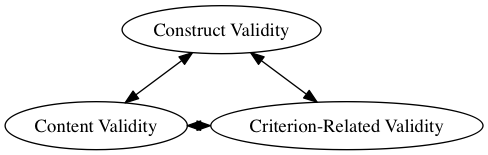
\includegraphics[scale=.5]{images/validity.png}}
}

\frame{
\frametitle{Overview of Validity}
\begin{itemize}
	\item \textcolor{Bittersweet}{Content} - Evaluation of subjects, topic, or content \textcolor{RoyalBlue}{covered by the items in the test}
	\item \textcolor{Bittersweet}{Criterion-Related} - \textcolor{RoyalBlue}{Evaluation relationship} of scores obtained on the test to scores on other instruments measuring the same construct
	\item \textcolor{Bittersweet}{Construct} - \textcolor{RoyalBlue}{Evaluation relationship} of scores obtained on the test to scores on other instruments measuring the same construct \textcolor{RoyalBlue}{AND} understanding how it fits within the \textcolor{RoyalBlue}{theoretical framework of the latent construct}
	\end{itemize}
}

\frame{
\frametitle{Face Validity is NOT Validity}
\centerline{
\includegraphics[scale=.5]{images/RodneyDangerfield_nofv.jpg}}
\vfill
{\footnotesize \href{https://upload.wikimedia.org/wikipedia/commons/b/bf/RodneyDangerfield1978.jpg}{source}
}}

\frame{
\frametitle{Content Validity}
\begin{itemize}
	\item How adequately the test represents the latent construct of interest
	\item Do the items throughly and completely tap into the latent construct?
	\item \textcolor{RoyalBlue}{How can we be sure I am teaching the entire domain of psychological testing?}
	\item Create a \textcolor{Bittersweet}{test blueprint} 
		\begin{itemize}
			\item What could be conceivably measured and in what proportion
		\end{itemize}
\end{itemize}
}

\frame{
\frametitle{Assessing Content Validity}
\begin{itemize}
	\item Assume you are giving an instrument to measure aggressive behavior in children
	\item \textcolor{RoyalBlue}{How can we assume this is measuring the construct of aggression?}
		\begin{itemize}
			\item Experts assess whether each item is essential to the definition of aggression
			\item $CVR = \frac{n_e - (N / 2)}{N / 2}$
			\item Where $n_e$ is number say ``essential" and N is number of experts
			\item Want this larger than chance (Table 6-1)
		\end{itemize}	 
\end{itemize}
}

\begin{frame}[fragile]
\frametitle{CVR in $R$}
\begin{itemize}
\item "Does your child bite other children?"
\item 20 experts, 17 say ``essential"
\end{itemize}
\begin{knitrout}
\definecolor{shadecolor}{rgb}{0.969, 0.969, 0.969}\color{fgcolor}\begin{kframe}
\begin{alltt}
\hlstd{CVR} \hlkwb{<-} \hlkwa{function}\hlstd{(}\hlkwc{e}\hlstd{,} \hlkwc{N}\hlstd{)\{}
        \hlstd{(e} \hlopt{-} \hlstd{(N} \hlopt{/} \hlnum{2}\hlstd{))}\hlopt{/}\hlstd{(N} \hlopt{/} \hlnum{2}\hlstd{)}
        \hlstd{\}}
\hlcom{# 17 say essential out of 20}
\hlkwd{CVR}\hlstd{(}\hlnum{17}\hlstd{,} \hlnum{20}\hlstd{)}
\end{alltt}
\begin{verbatim}
## [1] 0.7
\end{verbatim}
\end{kframe}
\end{knitrout}
\begin{itemize}
\item 0.7 $>$ 0.42
\end{itemize}
\end{frame}

\frame{
\frametitle{Assessing Content Validity}

\begin{center}
{\huge BUT ... expert judgement!!!}
\end{center}
}

\frame{
\say{Who controls the past controls the future; who controls the present controls the past.}

\vspace{1cm}
\centerline{
\includegraphics[scale=.5]{images/orwell.jpg}}

\vfill
{\footnotesize \href{https://c2.staticflickr.com/4/3463/3730530834_31d8f32a3b.jpg}{source}
}
}

\frame{
\frametitle{Criterion-Related Validity}
\begin{itemize}
	\item What the test score tells you about where a person falls on the underlying construct being measured w.r.t a criterion 
	\item  A \textcolor{Bittersweet}{criterion} is a benchmark or standard used for comparison
	\item Score high on an instrument measuring depression, \textit{but do you really have depression}?
	\item Show no symptoms of depression, instrument is \textcolor{RoyalBlue}{irrelevant} and \textcolor{RoyalBlue}{invalid}  
\end{itemize}
}

\frame{
\frametitle{Measuring Depression}
\begin{itemize}
	\item Predict whether someone is receiving counseling services based on Beck Depression Inventory
	\item Find out BDI was used to determine whether someone should receive services
	\item \textcolor{RoyalBlue}{What is wrong with this?} 
\end{itemize}
}

\frame{
\frametitle{Forms of C-R Validity}
\begin{itemize}
\item \textcolor{Bittersweet}{Concurrent Validity}
	\begin{itemize}
		\item Instrument provides the same ``scores" as an already validated measure
		\item Instruments must be administered at the same time (or nearly so)
		\item Example?
	\end{itemize}
\item \textcolor{Bittersweet}{Predictive Validity}
	\begin{itemize}
		\item How well an instrument predicts some criterion in the future
		\item SAT should measure ``college success"
		\item So it should be highly correlated with?
	\end{itemize}
\item 	\textcolor{Bittersweet}{validity coefficient}: an ``appropriate" measure of association
\end{itemize}
}

\frame{
\frametitle{Validity Coefficient}
\begin{itemize}
	\item In summary, everything that affects the correlation coefficient!
	\item Range restriction from attrition in a study or self-selection  
	\item Make sure testtakers are relevant in the validation study and cover the scope of the test! 
	\item Read the test manual and make sure test is appropriate for your testtakers 
	\item \textcolor{RoyalBlue}{Coefficient should be high enough to matter}
\end{itemize}
}

\frame{
\frametitle{Incremental Validity}
\begin{itemize}
	\item Want to predict final grade in first math class in college.
	\item Add most important predictor first (maybe SAT math score if in the USA)
	\item Then add additional variables, incrementally, and see what each predictor adds
	\item This is akin to stepwise regression in multiple regression
	\item \textcolor{RoyalBlue}{This is unwise because of inflation of type I error} (the probability of incorrectly rejecting a null hypothesis when you should have retained it)
\end{itemize}
}

\frame{
\frametitle{Construct Validity}
\begin{itemize}
	\item Evidence supporting that the test measures the underlying construct and that it can spread testtakers along that construct
	\item A test maker has theories about the construct, it's definition, structure, and relationship to other constructs and has theories about how their test relates to other tests
	\item All forms of validity are really subsumed within construct validity 
\end{itemize}
}

\frame{
\frametitle{Types of Construct Validity}
\begin{itemize}
	\item \textcolor{Bittersweet}{Homogeniety}
		\begin{itemize}
			\item Structure of a test should be homogeneous if it is measuring a single construct
			\item Responses to test items should be positively correlated with total score on the test
			\item Items that are not need to be removed or rewritten
		\end{itemize}
	\item Change with \textcolor{Bittersweet}{age} and  \textcolor{Bittersweet}{pre/post}
		\begin{itemize}
			\item Testtakers taking a test on algebra \textit{should} score higher if they are older
			\item Students getting tutored in algebra between a pre and post test should score higher on the post test
		\end{itemize} 
\end{itemize}
}

\frame{
\frametitle{Types of Construct Validity}
\begin{itemize}
	\item Groups higher on the construct should have higher scores
		\begin{itemize}
			\item Administer a test measuring tendency toward violent behavior
			\item Higher scores on test: General population or prison inmates for assault and battery
		\end{itemize}
\end{itemize}
}

\frame{
\frametitle{Factor Analysis}
\centerline{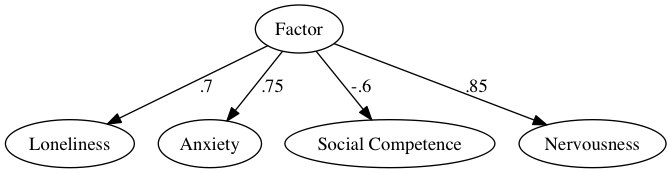
\includegraphics[scale=.5]{images/factor.png}}
\begin{itemize}
\item What should we call this factor?
\item If Nervousness is our new instrument to measure the factor, how well does it do?
\item What does it mean that social competence is negatively correlated with our factor?
\end{itemize}
}

\frame{
\frametitle{Test Bias and Fairness}
\begin{itemize}
	\item Test bias - degree to which a test systematically favors one group or another
	\begin{itemize}
		\item Can test for this statistically using logistic regression model
		\item  Known as \textcolor{Bittersweet}{differential item functioning}
	\end{itemize}
	\item Test fairness - the degree to which a test is fair and used in an equitable way
		\begin{itemize}
			\item Administer a test to a group not involved in the validation sample
			\item Maybe some groups of people are just different?
		\end{itemize}
\end{itemize}
}
\end{document}
